\documentclass[11pt,a4paper]{article}
\usepackage[margin=25mm]{geometry}
\usepackage{fontspec}
\setmainfont{texgyrepagella-regular.otf}[BoldFont=texgyrepagella-bold.otf,ItalicFont=texgyrepagella-italic.otf,BoldItalicFont=texgyrepagella-bolditalic.otf]
\usepackage[dutch]{babel}
\usepackage{microtype,amsmath,amssymb,booktabs,longtable,array,tabularx,ragged2e}
\usepackage{tikz}
\usetikzlibrary{arrows.meta,positioning}
\usepackage[backend=bibtex,style=authoryear,sorting=nyt,maxcitenames=2,maxbibnames=30,doi=true,url=true,isbn=false]{biblatex}
\addbibresource{references.bib}
\usepackage{xurl}
\usepackage[hidelinks,unicode]{hyperref}
\newcolumntype{P}[1]{>{\RaggedRight\arraybackslash}p{#1}}
\setlength{\emergencystretch}{4em}
\renewcommand{\arraystretch}{1.16}
\newcommand{\claim}[1]{\textsuperscript{\hyperref[app:claims]{\scriptsize #1}}}
\title{Master Data Management: concepten, capabilities en standaarden\\\large Een kritische literatuur- en standaardsynthese met aandacht voor de Nederlandse overheid}
\author{Onderzoeksmanuscript}
\date{9 september 2026\\\small Beschrijvende overzichtsstudie op basis van een afgebakend corpus}
\begin{document}
\maketitle
\begin{abstract}
Master Data Management (MDM) wordt besproken als technische integratievoorziening, organisatorische discipline en onderdeel van bredere data-architecturen. Deze paper onderzoekt hoe de belangrijkste concepten, capabilities, architectuurpatronen, governancebenaderingen en standaarden zich tot elkaar verhouden. De studie combineert een verkennende literatuurreview, analyse van officiële standaarddocumenten en conceptuele synthese. De initiële verwervingssnapshot omvat 96 bronvermeldingen en 178 bruikbare bestanden; deze aantallen zijn geen aantallen onafhankelijke studies. Relevante passages zijn doelgericht geselecteerd en beoordeeld. De studie claimt geen uitputtende systematische review, onafhankelijke dubbele screening of clausuledekkende normanalyse. De synthese onderscheidt entiteit, record, selectie van voorkeurswaarden, metadata, referentiedata en dataproduct, en ordent capabilities naar hun functie in de datalifecycle. Vroege MDM-bronnen behandelen reeds bedrijfssemantiek, context en masterdata als product. Daarom is een algemene tegenstelling tussen traditioneel MDM en semantisch of productgericht datamanagement niet houdbaar binnen dit corpus. De standaardenanalyse laat verschillende verantwoordelijkheden zien voor terminologie, modellering, registratie, kwaliteit, herkomst, catalogisering en uitwisseling. Hun gezamenlijke toepassing vraagt expliciete mappings en toepasselijkheidsbesluiten, maar rechtvaardigt niet vanzelf een nieuwe architectuur. Voor de Nederlandse overheid worden gezag, scope en standaardstatus afzonderlijk behandeld. Kennishiaten betreffen onder meer de vergelijkbaarheid van capability-taxonomieën, de voorwaarden waaronder semantische formalisering meerwaarde heeft en de verhouding tussen federatie en beheerlast. AI is één afnemer binnen dit landschap; prestatieverbetering en het voorkomen van onjuiste antwoorden worden niet als bewezen effecten gepresenteerd. Het bestaande prototype speelt geen rol in selectie, analyse of conclusies.
\end{abstract}
\noindent\textbf{Trefwoorden:} masterdata; Master Data Management; data governance; metadata; semantische interoperabiliteit; standaarden; literatuursynthese.
\newpage
\tableofcontents
\newpage
\section{Inleiding}
Master Data Management betreft in de onderzochte literatuur zowel het beheren van gegevens over belangrijke bedrijfsentiteiten als het organiseren van de verantwoordelijkheden die dat beheer mogelijk maken. De functionele MDM-studie van Otto en Ofner behandelt modellering, beschikbaarstelling, kwaliteit, onderhoud en archivering als samenhangende activiteiten. Een functioneel referentiemodel voor masterdatakwaliteit positioneert systeemondersteuning bovendien binnen een organisatorisch kwaliteitsvraagstuk. Daarmee is MDM geen synoniem voor een database of softwarepakket. \parencite{L20,L05}\claim{RC01}

De terminologie wordt complexer wanneer MDM in verband wordt gebracht met knowledge graphs, data products, Data Mesh en federatieve datastelsels. De literatuur onderscheidt deze benaderingen naar doel en organisatievorm, maar gebruikt ook overlappende begrippen. Blohm et al. bespreken expliciet de onderlinge samenhang van data products, data mesh en data fabric; Gieß en Hutterer vergelijken bredere datamanagementbenaderingen. Zulke vergelijkingen vormen antecedenten voor deze studie, geen bewijs dat al hun conclusies naar ieder MDM-domein kunnen worden overgedragen. \parencite{L12,L24}\claim{RC02}

Het onderzoeksdoel is de beschikbare kennis te structureren zonder een gewenste oplossing voorop te stellen. De bijdrage ligt in het onderscheiden van analyse-eenheden, het vergelijken van bronafhankelijke terminologie en het verbinden van capabilities met hun normatieve en organisatorische context. Het Stelsel van Basisregistraties biedt een toepassingsperspectief op gezag en gedeeld gegevensgebruik, maar deze paper is geen implementatiecasus of effectstudie.

\subsection{Onderzoeksvraag en deelvragen}
De hoofdvraag luidt: \emph{Wat is de huidige stand van wetenschappelijke, normatieve en professionele kennis over Master Data Management binnen het onderzochte corpus, en hoe hangen de belangrijkste concepten, capabilities, standaarden, architecturen en governancebenaderingen samen?}

De toevoeging ``binnen het onderzochte corpus'' begrenst de aanspraak op actualiteit en volledigheid. Zes deelvragen bundelen de 22 vraagthema's uit de onderzoeksopdracht:
\begin{enumerate}
\item OV1: hoe worden masterdata en verwante dataconcepten gedefinieerd, en welke historische en theoretische perspectieven zijn herkenbaar?
\item OV2: welke businessproblemen, capabilities, lifecycleactiviteiten en architectuurpatronen worden beschreven?
\item OV3: hoe worden identiteit, kwaliteit, governance, temporaliteit en herkomst behandeld?
\item OV4: welke rollen spelen metadata, semantiek, ontologie en standaarden, en waar ontstaan overlap, mappings of interpretatieverschillen?
\item OV5: hoe verhouden Nederlandse overheidskaders en ontwikkelingen rond dataproducten, federatie en AI zich tot MDM?
\item OV6: welke synthese is gerechtvaardigd, welke controverses blijven bestaan en welke vragen vereisen aanvullend onderzoek?
\end{enumerate}

\section{Onderzoeksmethode}
\subsection{Reviewstrategie en corpus}
De studie is een verkennende state-of-the-art review met standards landscape analysis en conceptuele synthese, voorbereid vanuit een scoping-reviewprotocol. PRISMA-ScR ondersteunt het expliciteren van doel, selectie en rapportage van scoping reviews; PRISMA-S richt zich op transparante rapportage van zoekactiviteiten. Deze paper gebruikt die aandachtspunten, maar claimt geen volledige naleving van alle rapportage-items of een retrospectief gereconstrueerde systematische review. \parencite{M01,M02}\claim{RC03}

De verwerving van 8 september 2026 bouwde voort op 70 bestaande vermeldingen: 51 standaard-/kadervermeldingen en 19 literatuurvermeldingen. Gerichte zoekacties voegden 26 kandidaten toe. De lokale verzameling bevat 90 PDF's en 88 webdocumenten, afkomstig van 218 geregistreerde downloadroutes. Er zijn 171 verschillende bestandshashes. Deze administratieve aantallen beschrijven beschikbaar materiaal: een standaard kan meerdere bijlagen hebben en één publicatie kan meerdere bron-ID's dragen. FAIR (S46/L11) en OntoClean (S50/L10) leveren bijvoorbeeld geen onafhankelijk dubbel bewijs. Tijdens de paperfase zijn drie afzonderlijke officiële statusbronnen toegevoegd en zijn Europese brondocumenten gericht aangevuld. Deze aanvullingen vallen buiten de genoemde verwervingssnapshot. Veertig routes leverden geen bruikbaar brondocument op; andere routes konden voor dezelfde bron wel slagen.

Zoekacties richtten zich op MDM-reviews, boeken, entity resolution, governance, Data Mesh, ontology engineering en officiële standaardpublicaties. Het zoeklog bevat de werkelijk gebruikte queries en geselecteerde vindplaatsen. Er is geen volledige databasebrede export of gedocumenteerde beoordeling van alle gerangschikte zoekresultaten. De eerdere bronselectie had een ontwerpgerichte aanleiding; de huidige studie behandelt die selectie als mogelijk vertekenend startbestand, niet als onafhankelijke afspiegeling van het vakgebied.

\subsection{Selectie, extractie en analyse}
Bronnen zijn inhoudelijk gebruikt wanneer zij een deelvraag ondersteunen en relevante tekst of een duidelijk begrensd officieel abstract beschikbaar is. Hoofdpublicatie, auteursversie, boekfragment, catalogus en gelinkte bijlage zijn onderscheiden. Bij downloads die via een standaardpagina zijn gevonden, is niet aangenomen dat de inhoud zelf tot die standaard behoort. Niet-gebruikte kandidaten blijven zichtbaar in het selectieregister.

De analyse-eenheid is een passage over een definitie, functie, relatie, patroon of toepassingsvoorwaarde. De extractie registreert bron-ID, bestand, hash, locatie, inhoudelijke parafrase en interpretatiegrens. De bronnen zijn doelgericht op de vraagthema's gelezen; de paper claimt geen integrale lezing van alle 178 bestanden. Boeken achter toegangsbeperkingen worden alleen aangehaald voor het geraadpleegde fragment of de officiële scopebeschrijving. Voor ISO en NEN ontbreekt grotendeels volledige normtoegang. Dat beperkt de analyse tot geregistreerde onderwerpen en niet tot uitputtende clausuleconformiteit.

De synthese vergelijkt eerst de bedoelde eenheden, vervolgens het abstractieniveau en daarna de normatieve of descriptieve functie. Bronafhankelijke definities blijven naast elkaar staan wanneer equivalentie niet kan worden onderbouwd. Een tweede analysegang zoekt tegenargumenten voor een veronderstelde tegenstelling tussen klassiek MDM en semantisch of productgericht datamanagement. Het claims-register scheidt normatieve uitspraken, claims met één of meerdere bronnen en eigen synthese. ``Meerdere bronnen'' betekent geen automatische consensus.

Er is geen onafhankelijke dubbele screening of interbeoordelaarsbetrouwbaarheid vastgesteld. De analyse en redactionele ondersteuning zijn door een AI-assistent uitgevoerd; een menselijke vakinhoudelijke review is nog nodig. De toegevoegde extracties en traceability maken de keuzes controleerbaar, maar vervangen die review niet. Geen prototype, gebruikersproef of AI-benchmark maakt deel uit van de methode.

\section{Definitie van Master Data}
Loshin verbindt masterdata met representaties van veelgebruikte bedrijfsconcepten en met een organisatiebrede, consistente blik op die informatie. Otto en Ofner onderscheiden masterdataklasse, attribuut en object, terwijl Wang et al. herhaald gebruik van kernentiteiten over bedrijfsprocessen en systemen benadrukken. Deze accenten wijzen op samenhang, maar leveren geen universele lijst van intrinsieke data-eigenschappen. \parencite{B01,L20,L18}\claim{RC04}

Voor deze synthese betekent \emph{masterdata}: gegevens over domeinentiteiten die binnen een vastgestelde organisatorische context herhaald worden gebruikt en waarvoor afgestemd beheer relevant is. Dit is een analytische werkdefinitie. Zij schrijft geen centrale opslag, unieke recordrepresentatie of bepaald update-interval voor. Een entiteit is hier de bedoelde referent; een record is een geregistreerde beschrijving daarvan. Meerdere records kunnen dezelfde referent beschrijven zonder inhoudelijk identiek te zijn.

Het onderscheid is van belang bij termen als \emph{master record} en \emph{golden record}. Een master record kan in een bron een aangewezen beheerrecord betekenen; golden record duidt veelal op een geïntegreerde selectie van gegevens uit bronnen. Gualo et al. gebruiken het laatste begrip in hun behandeling van masterdatarepositories. De toepasselijke selectie- en kwaliteitsregels blijven echter nodig om te bepalen wat zo'n record vertegenwoordigt. Het woord ``golden'' levert op zichzelf geen onafhankelijk bewijs van juistheid of bevoegd gezag. \parencite{L19,P01}\claim{RC05}

\section{Ontwikkeling en theoretische perspectieven}
Loshin beschrijft de ontwikkeling van MDM vanuit verspreide applicaties en uiteenlopende representaties van bedrijfsconcepten. Deze historische lezing is een professionele reconstructie, geen door deze paper uitgevoerde geschiedschrijving. Een precieze oorsprongsdatum van MDM wordt daarom niet vastgesteld. \parencite[§1.2]{B01}

De geselecteerde publicaties ondersteunen wel een reeks gedateerde ankerpunten. SMDM demonstreerde in 2009 semantische toegang tot masterdata. In 2011 beschreven Otto en Ofner strategische requirements, inclusief masterdata als product en business semantics management. Gualo et al. publiceerden in 2023 een kwaliteitsmodel voor masterdatarepositories. Recente syntheses verbreden vervolgens de vergelijking met data products en federatieve organisatievormen. Deze ankerpunten tonen continuïteit en variatie; zij bewijzen geen universele opeenvolging van volwassenheidsfasen. \parencite{L18,L20,L19,L12,L24}\claim{RC06}

Vier theoretische perspectieven zijn analytisch te onderscheiden. Het informatiekwaliteits-perspectief onderzoekt geschiktheid voor gebruik; het governanceperspectief onderzoekt bevoegdheden en besluitvorming; het integratieperspectief behandelt identificatie en afstemming tussen representaties; het ontologische perspectief onderzoekt aannames over objecten, categorieën en identiteit. Deze indeling is een synthese van de geselecteerde literatuur, geen bestaande uniforme MDM-theorie. Zij verklaart waarom een technisch succescriterium, zoals minder duplicaten, niet alle governance- of betekenisvragen beantwoordt. \parencite{L15,L07,L21,L08}\claim{RC07}

\section{Masterdata versus gerelateerde dataconcepten}
Datacategorieën moeten op hun classificatiegrond worden vergeleken. ``Operationeel'' en ``analytisch'' beschrijven in MDM-literatuur gebruiksscenario's; ``masterdata'' beschrijft een beheerd gegevensdomein. Een dataset is een publiceerbare verzameling, terwijl een dataproduct ook doel en consumptie adresseert. Daarom zijn deze labels niet allemaal wederzijds uitsluitende soorten data. \parencite{L20,S47,L12}\claim{RC08}

\begin{longtable}{@{}P{.19\linewidth}P{.37\linewidth}P{.36\linewidth}@{}}
\toprule Begrip & Analytische afbakening & Te vermijden gelijkstelling \\\midrule
Transactionele data & Beschrijven gebeurtenissen of handelingen; masterdata kunnen ernaar worden verwezen. & ``Transactional MDM'' is niet automatisch beheer van alle bedrijfsgebeurtenissen. \\
Referentiedata & Waardenstelsels voor toegestane of gedeelde classificaties; brongebruik kan ruimer zijn. & Niet ieder waardenstelsel is een entiteitenregister. \\
Metadata & Beschrijven gegevens, representatie of beheercontext. & Metadata zijn geen synoniem voor alleen technische schemas. \\
Operationele/\allowbreak analytische data & Gebruik in uitvoering respectievelijk analyse. & Masterdata kunnen beide soorten gebruik ondersteunen. \\
Dataset & Afgebakende gegevensverzameling in cataloguscontext. & Geen organisatieverantwoordelijkheid door het label alleen. \\
Dataproduct & Beheerd aanbod gericht op een terugkerende informatiebehoefte. & Kan master-, referentie- of andere data bevatten. \\
\bottomrule
\end{longtable}
De tabel is een werkordening op basis van de onderscheiden gebruikscontexten. De referentiedatabespreking in Gualo et al. omvat bijvoorbeeld zowel toegestane waarden als procedures om geldige waarden te bepalen. Die ruime formulering mag niet ongemotiveerd tot algemene definitie worden verheven. \parencite{L19,S08,S47,L12}

\section{MDM-capabilities en lifecycle}
Een capability wordt hier opgevat als een vermogen om een terugkerende beheertaak uit te voeren. Dat vermogen kan mensen, afspraken en software omvatten. De term wordt gebruikt om bronnen vergelijkbaar te maken, niet om te suggereren dat iedere auteur dezelfde taxonomie hanteert. Otto en Ofner beschrijven requirements op strategisch en functioneel niveau; het MDQM-referentiemodel organiseert systeemfuncties; de IBM-publicatie beschrijft implementatie- en modelleeractiviteiten. Hun granulariteit verschilt. \parencite{L20,L05,P01}\claim{RC09}

De onderstaande taxonomie groepeert brononderbouwde functies. Zij is niet gerangschikt naar volwassenheid en bevat geen universele aanschaflijst. Brede labels als observability en data product management zijn herkenbaar als hedendaagse ordening van eerder beschreven taken, niet als bewijs dat die taken pas recent ontstonden.

\begin{longtable}{@{}P{.19\linewidth}P{.43\linewidth}P{.30\linewidth}@{}}
\caption{Capability-taxonomie als synthese, met bron- en reikwijdtegrenzen.}\label{tab:capabilities}\\
\toprule Cluster & Functies & Bronbasis en begrenzing \\\midrule\endfirsthead
\toprule Cluster & Functies & Bronbasis en begrenzing \\\midrule\endhead
Governance & Eigenaarschap, stewardship, escalatie, workflow en goedkeuring. & \textcite{L20,L07}; rol- en besluitrechten zijn organisatieafhankelijk. \\
Identiteit & Identifierbeheer, entity resolution, matching en deduplicatie. & \textcite{L21,L29,S38}; een identifier is geen matchingalgoritme. \\
Consolidatie & Survivorship, samenvoeging, herstel van onjuiste samenvoeging en verrijking. & \textcite{P01,L22}; herstel als analytische foutafhandeling, niet overal gelijk benoemd. \\
Structuur & Hiërarchieën, relaties, reference data en datamodellering. & \textcite{P01,L19,S13}; technisch en domeininhoudelijk beheer onderscheiden. \\
Kwaliteit & Profilering, business rules, validatie en kwaliteitsmeting. & \textcite{L19,S32,S34}; formele geldigheid is slechts één kwaliteitsaspect. \\
Betekenis & Metadata management, begripsbeheer en semantische mappings. & \textcite{S08,S14,L18}; formalisering is een mogelijke uitwerking. \\
Verandering & Versioning, history, provenance en lineage. & \textcite{L14,S33,L20}; verschillende tijd- en herkomstvragen. \\
Beveiliging & Security, access control en rolgebonden toegang. & \textcite{L20,S21}; standaardscope bepaalt welk deel wordt ondersteund. \\
Distributie & Publicatie, synchronisatie, API management en eventing. & \textcite{P02,S19,S22}; interfaces zijn geen volledige governance. \\
Gebruiksbeheer & Gebruiksmonitoring, auditinformatie en productbeschrijving. & \textcite{L20,S51}; geen generiek gevalideerd observabilitymodel afgeleid. \\
\bottomrule
\end{longtable}

Het lifecyclepad identificeren, registreren, valideren, matchen, consolideren, verrijken, goedkeuren, publiceren, distribueren, wijzigen, historiseren en archiveren/verwijderen dient als analysekader. Niet iedere bron schrijft deze volgorde voor. Matching kan bijvoorbeeld vóór registratie in een hub gebeuren, of later tijdens herstel. Beheer is cyclisch waar correcties nieuwe validatie, publicatie en beoordeling vereisen. Dat is een procesmatige synthese van de beschreven activiteiten, geen nieuw normatief lifecyclemodel. \parencite{L20,P01,P02}\claim{RC10}

\begin{longtable}{@{}P{.21\linewidth}P{.31\linewidth}P{.40\linewidth}@{}}
\toprule Fasegroep & Verantwoordelijkheidsvraag & Te onderzoeken metadata, kwaliteit en ondersteuning \\\midrule
Identificeren/\allowbreak registreren & Wie bepaalt welke referent en bron worden bedoeld? & Identifiers, broncontext en registratievoorwaarden; invoer- en validatiefuncties. \\
Valideren/\allowbreak matchen & Wie stelt regels en beslisdrempels vast? & Regelversie, matchbewijs en foutcategorieën; algoritme en menselijke beoordeling. \\
Consolideren/\allowbreak verrijken & Wie mag voorkeurswaarden of relaties vaststellen? & Selectieregels, herkomst en onzekerheid; survivorship en herstelmogelijkheid. \\
Goedkeuren/\allowbreak publiceren & Wie neemt het vrijgavebesluit? & Besluit, versie, doelgroep en beperkingen; workflow en publicatiecontract. \\
Distribueren/\allowbreak wijzigen & Wie ontvangt welke verandering? & Interface, wijzigingstype en afhankelijkheden; synchronisatie en notificatie. \\
Historiseren/\allowbreak afsluiten & Welke toestand moet behouden of verwijderd worden? & Tijdassen, bewaarbeleid en aantoonbare intrekking; historie- en archieffuncties. \\
\bottomrule
\end{longtable}
Deze fasevragen zijn eigen vergelijkingsvragen voor corpusanalyse. Zij mogen niet als empirisch aangetoonde standaardwerkwijze van alle MDM-organisaties worden gelezen.

\section{Bestaande MDM-architectuurpatronen}
Architectuurtermen zijn niet consistent tussen bronnen. Otto en Ofner onderscheiden central system, leading system, repository en peer-to-peer. De IBM-modelleerpublicatie noemt external reference, registry, coexistence en centralized. Deze namen classificeren deels andere eigenschappen: locatie van gegevens, aanwijzing van een leidend systeem en organisatie van synchronisatie. Een namenlijst alleen levert daarom geen betrouwbare patroonmapping. \parencite{L20,P01}\claim{RC11}

\begin{longtable}{@{}P{.17\linewidth}P{.33\linewidth}P{.42\linewidth}@{}}
\caption{Vergelijking op schrijfverantwoordelijkheid en gegevensplaatsing; geen universele patroonstandaard.}\\
\toprule Patroonlabel & Kern van de beschrijving & Afweging en begrenzing \\\midrule\endfirsthead
\toprule Patroonlabel & Kern van de beschrijving & Afweging en begrenzing \\\midrule\endhead
Registry & Verwijzingen en identiteitskoppelingen; gegevens blijven in bronsystemen. & Beperkt kopiëren; beantwoording kan bronbeschikbaarheid en resolutie vragen. Virtuele deduplicatie verwijdert bronduplicaten niet. \\
Consolidation & Samenbrengen voor een geïntegreerde representatie of analyse. & Een uniforme afnamevorm is mogelijk; terugkoppeling naar bronnen volgt niet automatisch. \\
Coexistence & Gegevens bestaan zowel lokaal als in een hub; synchronisatie is nodig. & De IBM-bron laat bronnen als primair gelden. De term alleen bewijst dus geen tweezijdig schrijfgezag. \\
Centralized / transactional & Onderhoud van masterdata verschuift naar een leidende centrale voorziening. & Gecoördineerde mutatie; organisatorische overdracht van beheer moet worden geregeld. ``Transactional'' betreft hier masterdatamutaties. \\
Federated / peer-to-peer & Beheer en afstemming over meerdere organisatorische of technische eenheden. & Lokale autonomie en gezamenlijke afspraken moeten worden onderscheiden; peer-to-peer is niet vanzelf een volledig federatief governancemodel. \\
\bottomrule
\end{longtable}
De beschrijvingen zijn gebaseerd op \textcite{P01,L20,L23}; de aangegeven gevolgen zijn architectuurinterpretaties, geen gemeten rangorde. De specifieke betekenis van coexistence in de IBM-bron is een voorbeeld van waarom brongebonden definities behouden moeten blijven.

Voor een vergelijking zijn minstens acht assen relevant: doel, gegevensplaatsing, write authority, eigenaarschap, synchronisatiemechanisme, zichtbaarheidsvertraging, distributie en betekenisafstemming. Een patroonlabel bepaalt geen consistency model in formele zin. Evenmin volgen latency of schaalbaarheid uit het woord ``federatief''. Zulke eigenschappen vereisen een concrete implementatie, werkbelasting en meetdefinitie. De huidige bronnen maken een algemeen prestatieranglijstje niet mogelijk. \parencite{P01,P02,L24}\claim{RC12}

\section{Identity en Entity Resolution}
Entity resolution onderzoekt of verschillende records naar dezelfde referent verwijzen. Getoor en Machanavajjhala plaatsen deze vraag op het raakvlak van onder meer databases, machine learning en informatieontsluiting. Een vergelijking van tekens is daarbij slechts een mogelijke stap. Blocking beperkt kandidaten, matching beoordeelt overeenkomsten en een daaropvolgend besluit bepaalt welke koppeling of clustering wordt aanvaard. \parencite{L21,L29,L30}\claim{RC13}

Een identifier werkt binnen een gekozen naamgevings- en uitgiftecontext. URI/IRI-specificaties en publicatieadviezen regelen aspecten van identificatie en verwijzing, maar beslissen niet of twee administratieve registraties dezelfde domeinentiteit bedoelen. Daarom moeten identifiergelijkheid, recordgelijkheid en referentidentiteit afzonderlijk worden geanalyseerd. De juridische of institutionele betekenis van de referent kan bovendien per domein verschillen. \parencite{S38,S39,L08}\claim{RC14}

Survivorship betreft de keuze van te gebruiken waarden wanneer bronnen verschillen. Een matchbesluit zegt nog niet welke waarde voor welk doel moet gelden. Evenzo kan een samenvoeging achteraf onjuist blijken. Een split kan een correctie van een cluster zijn, maar in een domein ook een verandering van het object zelf beschrijven. Deze twee betekenissen zijn analytisch te onderscheiden; een productfunctie met de naam ``split'' zegt niet welke ervan wordt ondersteund. \parencite{P01,L22,L08}\claim{RC15}

De keuze van evaluatiemaatstaf is inhoudelijk relevant. Menestrina et al. laten zien dat entity-resolutionmaten dezelfde uitkomsten verschillend kunnen rangschikken. Pairwise- en clustermaatstaven beschrijven niet noodzakelijk dezelfde foutkosten. Voor publieke toepassingen kan een onterechte samenvoeging andere gevolgen hebben dan een gemiste koppeling; die asymmetrie is een te expliciteren toepassingskeuze, geen in deze paper gemeten overheidsuitkomst. \parencite{L22}\claim{RC16}

\section{Data Quality}
Datakwaliteit omvat meer dan juistheid van afzonderlijke waarden. Het consumentenperspectief van Wang en Strong en de vergelijking van kwaliteitsdimensies bij Gualo et al. maken duidelijk dat verschillende doelen en contexten verschillende beoordelingsaspecten vragen. Gualo et al. ontwikkelen een model met standaardaanknopingspunten en demonstreren toepassing in een repositorycasus. Hun studie ondersteunt het bestaan van een operationalisering; zij bewijst geen universele geschiktheid voor ieder MDM-domein. \parencite{L15,L19}\claim{RC17}

In deze analyse wordt validiteit gebruikt voor voldoen aan een gekozen regel of domein, volledigheid voor dekking van vereiste gegevens, consistentie voor het ontbreken van relevante tegenstrijdigheden, actualiteit voor temporele bruikbaarheid en juistheid voor overeenkomst met de bedoelde werkelijkheid of gezaghebbende beoordelingsgrond. Deze beknopte omschrijvingen zijn vergelijkingsconventies. Zij vervangen niet de afzonderlijke definities in ISO/IEC 25012 of andere bronnen. \parencite{S12,L19}\claim{RC18}

ISO 8000 behandelt onder meer masterdata-uitwisseling en semantische codering. ISO/IEC 25012 positioneert een datakwaliteitsmodel, terwijl DQV een vocabulaire biedt om kwaliteitsmetingen en context te beschrijven. SHACL ondersteunt controle van een datagraaf tegen vastgelegde shapes. Deze functies vullen elkaar aan, maar een geslaagde shapevalidatie toont niet dat een adres, identiteit of bevoegdheidsclaim feitelijk correct is. Dat laatste is een analytische gevolgtrekking uit de verschillende toetsobjecten. \parencite{S02,S03,S12,S32,S34}\claim{RC19}

De studie van Gualo et al. verwijst ook naar ISO/IEC 25024. Dit is een gemotiveerde uitbreidingsroute voor nader onderzoek naar meting, geen in deze paper onafhankelijk gelezen norm. Over de conformiteit met dat document worden daarom geen eigen uitspraken gedaan. Dezelfde terughoudendheid geldt wanneer een academische bron een normtitel of deelnummer onnauwkeurig weergeeft: het artikel vervangt dan niet de officiële normregistratie. \parencite{L19}

\section{Governance en Stewardship}
De officiële DAMA-DMBOK-pagina documenteert de herziene editie van dit professionele kenniswerk. Omdat de volledige boektekst niet is geraadpleegd, gebruikt deze paper DAMA-DMBOK niet als bewijs voor een uitputtende capability- of rol-taxonomie. Die beperking onderscheidt het professionele referentiekader van de inhoudelijk gebruikte artikelen en boekfragmenten. \parencite{S01}

Governance betreft in de review van Abraham et al. de uitoefening van gezag en controle over gegevensbeheer. De auteurs onderscheiden meerdere dimensies en mechanismen; hun conceptueel overzicht geeft geen enkel verplicht organisatiemodel. Voor MDM impliceert dit dat kwaliteit, toegang en betekenis ook besluitrechten en verantwoordelijkheden vereisen. De organisatorische taak kan niet worden afgeleid uit de opslaglocatie alleen. \parencite{L07,L20} De recente review van Guerreiro et al. stelt het verband tussen MDM-frameworks en governancevolwassenheid centraal. De auteurs plaatsen empirische validatie van hun conceptuele kader echter expliciet in vervolgonderzoek. Hun synthese wordt hier daarom gebruikt als verwant overzichtswerk, zonder er een causaal aangetoond effect van MDM op volwassenheid aan te ontlenen. \parencite{L27}\claim{RC20}

\begin{longtable}{@{}P{.20\linewidth}P{.38\linewidth}P{.34\linewidth}@{}}
\toprule Rolterm & Te analyseren verantwoordelijkheid & Bewijsgrens \\\midrule
Data owner & Beslissen over doelen, gebruik en verantwoord beheer. & Terminologie en mandaat verschillen per organisatie. \\
Data steward & Operationele coördinatie van kwaliteit, betekenis en issues. & Geen automatisch juridisch eigendom. \\
Custodian & Technische zorg voor opslag, bescherming en beschikbaarstelling. & Vergelijkingsrol; niet overal als aparte functie gedefinieerd. \\
Domain owner & Afbakening en afstemming binnen een gegevensdomein. & In federatieve benaderingen aan domeinorganisatie gerelateerd. \\
Product owner & Verantwoordelijkheid voor een beheerd aanbod aan afnemers. & Productverantwoordelijkheid verleent geen automatisch brongezag. \\
\bottomrule
\end{longtable}
Deze rolvergelijking ordent verantwoordelijkheidsvragen uit MDM-, governance- en dataproductliteratuur; zij is geen gezamenlijke definitie van alle bronnen. Vooral custodian en domain owner vragen verdere bronvergelijking voordat een uniforme rol-taxonomie kan worden gesteld. \parencite{L20,L07,L23,S51}\claim{RC21}

Governancevormen kunnen gecentraliseerde besluitvorming, gedelegeerde domeinverantwoordelijkheid en gezamenlijke regels combineren. BOMOS behandelt beheer van standaarden; het is daarmee relevant voor de afspraken waarop MDM steunt, maar geen volledige vervanging van organisatiebrede data governance. Het beheer van een standaard en het beheer van een gegevensverzameling hebben verschillende objecten en bevoegdheden. \parencite{S23,L07}\claim{RC22}

\section{Metadata en Data Elements}
Metadata verbinden een gegevensrepresentatie met informatie over betekenis, vorm of beheer. ISO/IEC 11179 adresseert metadataregistratie en maakt onderscheid tussen conceptuele en representatiegerichte constructies. Binnen het dossier is vooral het onderscheid tussen data-elementconcept en waardedomein relevant. De beschikbare officiële scope-informatie ondersteunt deze positionering, maar geen volledige beoordeling van alle modelclausules. De catalogus vermeldt bij ISO/IEC 11179-3:2023 tevens Amendment 1:2026 over item mappings; de inhoud daarvan is niet geanalyseerd. \parencite{S07,S08,S09,S10}\claim{RC23}

Een technisch veld met een naam en datatype bepaalt niet zelfstandig welke eigenschap van welk object wordt weergegeven. Een beschrijving kan daarnaast een definitie, context, eenheid, toegestane waarden en bronverwijzing nodig hebben. Welke daarvan noodzakelijk zijn, hangt af van de concrete interpretatietaak. Dit is een synthese van terminologie- en metadatawerk; geen eis dat iedere waarde alle context steeds in dezelfde payload moet meedragen. \parencite{S11,S08,S14}\claim{RC24}

Metadataregistries en datacatalogi hebben aanpalende, maar verschillende analyse-eenheden. Een metadataregistry kan dataspecificaties registreren; DCAT beschrijft onder meer datasets, distributies en dataservices. Een catalogusbeschrijving van een dataset is dus niet vanzelf een volledige beschrijving van ieder data-element. Omgekeerd geeft een verzameling elementdefinities nog geen compleet overzicht van het beschikbare aanbod. De grens is niet exclusief: ISO/IEC 11179-33 adresseert zelf datasetregistratie, inclusief kwaliteits- en herkomstmetadata. Er is dus daadwerkelijke overlap op datasetniveau; een tegenstelling tussen de gehele ISO/IEC 11179-serie en catalogisering zou te sterk zijn. \parencite{S08,S09,S47}\claim{RC25}

\section{Semantiek en Begrippen}
Een term is een aanduiding; een definitie beschrijft de afbakening van het bedoelde begrip. ``Begrip'' en ``concept'' kunnen vertaalvarianten zijn, maar bronnen kunnen ze ook op verschillende manieren in hun model gebruiken. De analyse behandelt ze daarom als afzonderlijke labels waarvan de relatie per bron wordt vastgesteld. Zij poneert niet vooraf dat begrip en concept twee universeel verschillende ontologische categorieën vormen. \parencite{S11,S13,S31}\claim{RC26}

SKOS biedt een model voor begrippenstelsels, labels en relaties. NL-SBB specificeert beschrijvingen van begrippen en werkt de relatie met informatiemodellen en begrippenbeheer uit. MIM behandelt verschillende beschouwingsniveaus en modelconstructies. Het zijn daarmee deels complementaire instrumenten, met expliciet beschreven raakvlakken. NL-SBB is niet eenvoudigweg overbodig omdat SKOS bestaat, en MIM is niet hetzelfde soort artefact als een afzonderlijk begrippenstelsel. \parencite{S31,S14,S13}\claim{RC27}

Een belangrijk tegenargument tegen een te scherpe oud/nieuw-tegenstelling komt uit het MDM-corpus zelf. Loshin bespreekt al uiteenlopende definities van gedeelde bedrijfsconcepten. Otto en Ofner noemen business semantics management en contextafhankelijke masterdata. Expliciete bedrijfsbetekenis is dus aantoonbaar onderdeel van sommige eerdere MDM-benaderingen. De resterende vraag is welke mate van formalisering en uitvoerbare koppeling wordt bereikt, niet of betekenis ooit onderwerp van MDM was. \parencite{B01,L20}\claim{RC28}

\subsection{Semantic false agreement}
Als twee systemen hetzelfde label gebruiken, kan hun schijnbare overeenstemming een verschillende afbakening verhullen. Omgekeerd kunnen verschillende labels hetzelfde bedoelen. Hier wordt \emph{semantic false agreement} gebruikt als analytische aanduiding van zulke onterecht aangenomen overeenstemming, niet als nieuw empirisch vastgesteld fenomeen of uniforme term van alle bronnen. De probleembeschrijving bij Loshin en de afzonderlijke label- en conceptconstructies in SKOS geven aanknopingspunten. \parencite{B01,S31}\claim{RC29}

Het onderscheid tussen syntactische, structurele en semantische interoperabiliteit helpt dit te analyseren. Syntactische overeenstemming betreft de leesbare representatie; structurele overeenstemming de ordening en modelrelaties; semantische overeenstemming de interpretatie. Organisatorische afstemming en juridische toepasselijkheid voegen andere voorwaarden toe. EIF onderscheidt juridische, organisatorische, semantische en technische interoperabiliteit; de uitsplitsing van syntaxis en structuur is hier een nadere analytische ordening binnen de technische en semantische bespreking, niet een letterlijke vijfdelige EIF-classificatie. \parencite{S43}\claim{RC30}

\section{Ontologie en Conceptual Modelling}
Een ontologische analyse onderzoekt welke categorieën en identiteitscriteria een model veronderstelt. In Guizzardi's werk worden dergelijke grondslagen gebruikt om structurele conceptuele modellen te beoordelen. Een objecttype dat bijvoorbeeld een rol representeert, kan andere identiteitsvoorwaarden hebben dan een type dat een zelfstandig object bedoelt. Het model maakt dus aannames over de referenten; deze aannames verdwijnen niet doordat het diagram technisch correct is. \parencite{L08}\claim{RC31}

UFO en OntoUML zijn relevant als ontologische grondslag respectievelijk modelleer\-benadering. OntoClean biedt een aanvullende manier om taxonomische beslissingen te beoordelen. Het zijn geen automatisch noodzakelijke voorzieningen voor ieder MDM-programma. OntoUML is bovendien geen Nederlandse overheidsstandaard. De afweging betreft de concrete modelleervraag, beschikbare expertise en gevolgen van foutieve categorie- of identiteitskeuzen. \parencite{S40,S41,L10}\claim{RC32}

Een ontologische klasse, MIM-objecttype, modelattribuut en data-element worden niet zonder mapping gelijkgesteld. Tegelijk verbiedt SKOS niet algemeen dat dezelfde resource ook als OWL-klasse wordt gebruikt. Een verantwoord onderscheid betreft hier de representatierol en interpretatieregels, niet een universele verplichting tot disjuncte resourceverzamelingen. \parencite[§3.5.1]{S31}\parencite{S13,S08}\claim{RC33}

\subsection{Knowledge graphs en Semantic Web}
RDF biedt een graafgebaseerde representatie; RDFS en OWL voegen verschillende semantische beschrijvingsmogelijkheden toe. JSON-LD biedt een JSON-gebaseerde representatie van linked data, terwijl SPARQL querymogelijkheden voor RDF adresseert. Deze bouwstenen kunnen samen worden gebruikt zonder dat zij één verplicht opslagproduct of één centrale database voorschrijven. \parencite{S28,S29,S30,S35,S36}\claim{RC34}

SMDM is een concreet antecedent: Wang et al. beschrijven virtuele RDF-toegang tot relationele masterdata, ontologieën, mappings en redeneerondersteuning. Dat ondersteunt de mogelijkheid van semantische uitbreiding van MDM en weerspreekt de nieuwheid van die combinatie als zodanig. De demonstratie onderbouwt geen algemene kosten-batenuitspraak voor alle organisaties of hedendaagse AI-toepassingen. \parencite{L18}\claim{RC35}

De kennisgraafliteratuur bespreekt uiteenlopende vormen van schema, identiteit, context en gevolgtrekking. Een knowledge graph is daarom geen garantie dat begrippen onderling zijn geharmoniseerd of gezagsclaims zijn gecontroleerd. Een foutieve mapping kan ook in een formeel valide graaf bestaan. Deze beperking volgt uit het onderscheid tussen representatie en de juistheid van de gemodelleerde inhoud. \parencite{L13,S32}\claim{RC36}

\section{Provenance, Lineage en Temporaliteit}
PROV-O onderscheidt entiteiten, activiteiten en agents en biedt relaties voor onder meer gebruik, generatie en afleiding. Daarmee kan herkomst in samenhang worden beschreven. Lineage wordt in deze paper gebruikt voor de gevolgde gegevens- en transformatieketen; provenance omvat daarnaast de context waarin zulke relaties worden verantwoord. Dit is een praktische werkafbakening, geen claim dat alle auteurs dezelfde terminologische grens hanteren. \parencite{S33}\claim{RC37}

Herkomst is niet hetzelfde als waarheid of bevoegdheid. Een bekende agent kan een onjuist gegeven produceren; een goed gedocumenteerde bewerking kan een inferentie opleveren die niet als authentiek brongegeven mag worden behandeld. Deze onderscheidingen zijn een conceptuele synthese van provenance en stelselverantwoordelijkheden. De aanwezigheid van een PROV-relatie bewijst niet zelfstandig de juridische grond van een uitspraak. \parencite{S33,S25}\claim{RC38}

Valid time betreft wanneer een feit geldt in de gemodelleerde werkelijkheid; transaction time wanneer het als actuele databasekennis is opgeslagen. De temporele databaseglossary maakt dit onderscheid expliciet. Een registratiecontext moet daarnaast aangeven op welk systeem een registratiemoment betrekking heeft. Het moment waarop een afnemer een record ontvangt is niet automatisch het transactiemoment van de bron. \parencite{L14}\claim{RC39}

OWL-Time adresseert temporele representatie, ISO 8601 datum- en tijdnotatie. Geen van beide kiest op zichzelf het beleid voor retroactieve correcties, versie-identiteit of bewaring. Die grens is relevant bij de interpretatie van historische masterdata: gelijke datumvelden betekenen nog geen gelijke tijdssemantiek. De IBM-bron behandelt geldigheidsintervallen en technische wijzigingshistorie bovendien al als verschillende aspecten van een MDM-model. \parencite{S37,S52,P01}\claim{RC40}

\section{Het standaardenlandschap}
\subsection{Documentsoorten en normatieve reikwijdte}
Het corpus bevat normen, technische specificaties, vocabularia, ontologieën, metamodellen, beheerhandreikingen, principes en wetgeving. Deze classificaties vormen verschillende assen. Een ontologie kan als W3C Recommendation zijn gepubliceerd; een metamodel kan een Nederlandse standaard zijn. FAIR is geen ISO-norm en de Interoperable Europe Act is geen vocabulaire. Zulke verschillen bepalen welke conclusies de bron kan ondersteunen. \parencite{S30,S13,L11,S42}\claim{RC41}

Het verschil tussen een normatieve passage en empirisch bewijs blijft eveneens essentieel. Een publicatie kan voorschrijven hoe gegevens worden uitgewisseld zonder te meten hoeveel interpretatiefouten daarmee verdwijnen. De aanwezigheid van een normatieve eis is geen effectstudie. Deze paper analyseert daarom toepassingsgebied en constructies afzonderlijk van claims over gerealiseerde voordelen.

\begin{longtable}{@{}P{.19\linewidth}P{.35\linewidth}P{.38\linewidth}@{}}
\caption{Cross-standard analyse: complementaire taken en de grenzen van de verbinding.}\label{tab:landscape}\\
\toprule Niveau / vraag & Relevante instrumenten & Aansluiting en grens \\\midrule\endfirsthead
\toprule Niveau / vraag & Relevante instrumenten & Aansluiting en grens \\\midrule\endhead
Terminologie & ISO 704, NL-SBB, SKOS & Begripsbeschrijving en begrippenrelaties; nog geen volledig logisch recordschema. \\
Ontologische analyse & UFO, OntoUML, OntoClean; OWL voor formalisering & Categorieën en axioma's; geen algemeen bewijs van noodzaak of optimale modellering. \\
Informatie\-modellen & MIM, NEN 3610, SEMIC Core Vocabularies & Modelconstructies en domeinhergebruik; mapping naar eigen begripscontext blijft nodig. \\
Metadata\-registratie & ISO/IEC 11179 & Betekenis en representatie van dataspecificaties; niet hetzelfde als een datasetcatalogus. \\
Masterdata\-kwaliteit & ISO 8000, ISO/IEC 25012 & Uitwisseling en kwaliteitsdimensies; volledige toepasselijke normtekst nodig voor clausuleanalyse. \\
Regels en metingen & SHACL, DQV & Graafvalidatie en kwaliteitsbeschrijving; geen garantie van feitelijke juistheid. \\
Herkomst en tijd & PROV-O, OWL-Time, ISO 8601 & Herkomststructuur, tijdsrelaties en notatie; gezag en historiebeleid niet automatisch bepaald. \\
Aanbod en producten & DCAT, DCAT-AP, DCAT-AP-NL, DPROD & Catalogusresources en productbeschrijving; geen uniforme definitie van ieder data-element. \\
Distributie & OpenAPI, REST API Design Rules, Digikoppeling, FSC & Interfaces en uitwisseling; betekenisafstemming vraagt aanvullende afspraken. \\
Wijzigingen & NL GOV CloudEvents & Eventbeschrijving en notificatie; geen volledige definitie van de domeinverandering. \\
Beheer en context & BOMOS, MDTO, EIF, overheidskaders & Standaardbeheer, duurzame toegankelijkheid en interoperabiliteit; verschillende beheerobjecten. \\
\bottomrule
\end{longtable}
De tabel is eigen synthese van de afzonderlijke bronposities; de appendix identificeert documentversies en beperkingen. Het is geen lijst van gezamenlijk verplichte componenten.\claim{RC42}

\subsection{Overlap, mappings en hiaten}
Drie relaties moeten uit elkaar worden gehouden. Ten eerste kan een profiel een bestaande standaard nader invullen, zoals DCAT-AP en DCAT-AP-NL rond DCAT. Ten tweede kunnen documenten verschillende aspecten van dezelfde resource beschrijven, zoals DQV en PROV-O voor kwaliteitsmetadata en hun herkomst. Ten derde kan een verbinding een onderzoekersmapping zijn, bijvoorbeeld tussen een lokaal begrip en een ontologische klasse. Alleen de eerste twee zijn door de genoemde standaarden rechtstreeks gepositioneerd; de derde vergt afzonderlijke rechtvaardiging. \parencite{S47,S45,S16,S34,S33,S31}\claim{RC43}

Het ontbreken van een onderwerp in één standaard is niet vanzelf een hiaat. OpenAPI hoeft niet alle institutionele identiteitscriteria te formaliseren om een bruikbare interfacespecificatie te zijn. Een inhoudelijke lacune ontstaat pas ten opzichte van een gemotiveerde behoefte én de gezamenlijk onderzochte dekking. Evenzo bewijst overlap geen redundantie: NL-SBB beschrijft ook gebruiks- en beheerafspraken die niet uit de loutere aanwezigheid van SKOS volgen. \parencite{S19,S14,S31}\claim{RC44}

\section{Nederlandse overheidscontext}
\subsection{Stelsel van Basisregistraties}
De historische eisen voor basisregistraties verbinden registratie met wettelijke verankering, verantwoordelijkheden, kwaliteit en terugmelding. De kwaliteitsbaseline werkt stelselbrede kwaliteitszorg verder uit. Deze bronnen zijn relevant voor MDM omdat zij laten zien dat gedeeld gebruik van kerngegevens niet losstaat van institutionele afspraken. De kwalificatie ``masterdata'' verleent op zichzelf echter geen authenticiteit of bevoegdheid. \parencite{S25,S26}\claim{RC45}

Het Stelsel kan niet zonder nadere analyse als één commerciële MDM-hub worden beschreven. Een vergelijking moet onderscheid maken tussen de verantwoordelijke registratie, de gegevensverstrekking en een eventuele samengestelde afnemersweergave. Dit is een toepassingsinterpretatie, geen claim dat alle basisregistraties op dezelfde technische wijze zijn ingericht. De paper onderzoekt geen operationele keten tussen registraties.

De BAG-catalogus biedt een concrete documentatiecontext met onder meer nummeraanduiding, verblijfsobject en pand. Een overeenkomstig label in een andere registratie bewijst geen identiteit. Voor een toekomstige vergelijking zijn brondefinities, modelrelaties en tijdsbetekenis nodig. Hier dient BAG uitsluitend om duidelijk te maken welke soorten documenten en begrippen bij een overheidsgerichte MDM-analyse moeten worden onderscheiden. Er worden geen niet-gecontroleerde BRP-, BRK- of WOZ-relaties ingevuld. \parencite{S49}\claim{RC46}

\subsection{Nederlandse modellen, begrippen en metadata}
MIM ordent conceptuele en logische informatiemodellering; NL-SBB ordent begripsbeschrijvingen; TOOI biedt een kennismodel voor overheidsinformatie. NEN 3610 vormt een afzonderlijke normatieve context voor geo-informatie. DCAT-AP-NL adresseert catalogusmetadata. Dit zijn verschillende abstractieniveaus en toepassingsgebieden, zodat een gezamenlijk gebruik niet mag worden teruggebracht tot een keuze voor één universele modeltaal. \parencite{S13,S14,S15,S17,S16}\claim{RC47}

Voor MDTO is het relevante vraagstuk duurzame toegankelijkheid en metagegevens van informatieobjecten. Het kan daardoor raken aan archivering en historie, maar is niet zonder meer een vervanging voor een masterdata- of begrippenmodel. BOMOS gaat juist over beheer van standaarden. De twee documenten delen een beheerthema zonder noodzakelijk hetzelfde beheerobject te hebben. \parencite{S24,S23}

\subsection{Versie, lijststatus en toepasselijkheid}
Bij de officiële lijstcontrole op 9 september 2026 is MIM 1.2 aanbevolen. De verplichte lijst vermeldt NL-SBB 1.0, OpenAPI Specification 3.0, REST API Design Rules 2.2 en NL GOV CloudEvents 1.1. DCAT-AP-NL 3.0 staat bij de standaarden in behandeling. Ook TOOI en MDTO staan op de geraadpleegde lijst in behandeling. Dit zijn waarnemingen van de officiële registraties op de peildatum, geen zelfstandig oordeel over iedere organisatie of gegevensuitwisseling. \parencite{F01,F02,F03}\claim{RC48}

De technische analyse gebruikt onder meer OpenAPI 3.1.1. Dat is een specificatieversie en niet automatisch de versie die op de Nederlandse lijst is vastgesteld. Formele status en technische documentversie worden daarom in de matrix gescheiden. De paper leidt uit de aanwezigheid op een lijst geen onvoorwaardelijke wettelijke verplichting voor alle MDM-functionaliteit af. \parencite{S19,F01,F03}

\subsection{Federatief Datastelsel en Europese kaders}
Het geraadpleegde FDS-afwegingskader vormt een ingang naar voorwaarden voor toelating van aanbod. De beschikbare hoofdpagina is echter onvoldoende om alle operationele afspraken van FDS inhoudelijk te reconstrueren. De studie positioneert FDS daarom als relevante Nederlandse onderzoekscontext en laat gedetailleerde vergelijking met federatieve MDM-patronen open. \parencite{S27}\claim{RC49}

EIF ordent interoperabiliteit over meerdere niveaus. De Interoperable Europe Act vormt een juridisch kader voor interoperabiliteit in de Europese publieke sector. SEMIC Core Vocabularies bieden herbruikbare kernmodellen, bijvoorbeeld voor personen, organisaties en locaties. Hun rol verschilt: een juridisch of bestuurlijk kader is geen datamodel, en een kernvocabulaire beslist niet automatisch over de volledige betekenis van een nationale registratierelatie. \parencite{S43,S42,S44}\claim{RC50}

FAIR benadrukt vindbaarheid, toegankelijkheid, interoperabiliteit en herbruikbaarheid, inclusief aandacht voor machinegericht gebruik. De principes ondersteunen daarmee het belang van metadata en expliciete verwijzingen. Zij verplichten niet alle gegevens openbaar te maken en bewijzen geen bepaalde MDM-architectuur. \parencite{L11}\claim{RC51}

\section{Masterdata en Data Products}
Dataproductdenken legt nadruk op een terugkerende informatiebehoefte, beheer en consumptie. Een dataproduct kan masterdata aanbieden, maar ook gegevens uit andere categorieën. De relatie is daarom geen eenvoudige vervanging van de ene term door de andere. Productdenken betreft het georganiseerde aanbod; masterdata betreft een gegevens- en beheervraagstuk dat daarbinnen kan liggen. \parencite{L12}\claim{RC52}

De gedachte dat masterdata als product kunnen worden behandeld is ouder dan de recente Data Mesh-discussie. Otto en Ofner noemen dit expliciet en verbinden er productbeschrijvingen en zicht op bronnen en afnemers aan. Een nieuw label is dus onvoldoende om een nieuwe capability of wetenschappelijke bijdrage te claimen. Wel blijft onderzoek nodig naar de praktische invulling en verschillen tussen oudere en recente productbenaderingen. \parencite{L20}\claim{RC53}

DPROD biedt een kandidaatvocabulaire voor productmetadata, waaronder eigenaar, doel en relaties met datasets en diensten. De hier geraadpleegde versie is 1.0 Beta 1. De bron ondersteunt het bestaan van een productspecificatie, niet dat deze versie iedere MDM-behoefte afdekt of dat een specifiek product ermee conformeert. Samenhang met DCAT-profielen en metadataregistries vraagt een vergelijking van resources en verantwoordelijkheden. \parencite{S51,S47,S08}\claim{RC54}

\section{Masterdata en federatieve data-architecturen}
De grijze-literatuurreview van Goedegebuure et al. synthetiseert praktijkmateriaal over Data Mesh. De beschreven principes betreffen domeinverantwoordelijkheid, data als product, self-service en federatieve governance. De geraadpleegde auteursversie is geen door deze paper uitgevoerd praktijkonderzoek; de onderliggende professionele claims worden niet automatisch bewijs van gerealiseerde voordelen. \parencite{L23}\claim{RC55}

Federatie betreft bovendien meerdere dimensies: verdeling van gegevens, verdeling van besluitrechten en de afspraken waarmee partijen samenwerken. Een centraal metadataoverzicht kan met decentraal gegevensbeheer samengaan. Daarom is een tegenstelling tussen ``centraal MDM'' en ``decentraal Data Mesh'' analytisch te grof. De patroonbeschrijvingen en recente architectuurvergelijkingen bevatten verschillende combinaties; de optimale keuze volgt daar niet algemeen uit. \parencite{L20,L23,L24}\claim{RC56}

Gieß en Hutterer ordenen data platforms, spaces, meshes en fabrics onder meer naar governance en toepassingsgebied. Hun synthese is bruikbaar als vergelijkingskader, maar een classificatie op dat niveau bepaalt geen formele consistentiegaranties of lokale beheerlast. Beheerautonomie kan extra afstemming vragen; centralisatie kan bevoegdheden bundelen. Beide zijn afwegingsdimensies die in een concrete context moeten worden onderzocht. \parencite{L24}

\section{API-first, events en data contracts}
OpenAPI beschrijft interfaces, de Nederlandse REST-regels stellen ontwerpafspraken en Digikoppeling/FSC adresseert onderdelen van gegevensuitwisseling en verbindingen. Het NL GOV-profiel voor CloudEvents beschrijft gebeurtenissen binnen een uitwisselingscontext. Deze instrumenten kunnen distributie en verandering ondersteunen, maar definiëren niet vanzelf de domeinbetekenis van een merge, correctie of intrekking. \parencite{S19,S18,S20,S21,S22}\claim{RC57}

``API-first'' en ``event-driven'' worden hier als ontwerporiëntaties onderzocht, niet als bewezen opvolgers van MDM. Hetzelfde geldt voor data contracts. De term kan een technisch schema, een kwaliteitsafspraak of een breder productcontract aanduiden. DPROD, catalogusprofielen en interfacespecificaties bieden aangrenzende constructies, maar het huidige corpus rechtvaardigt geen universele definitie of rangorde van data-contractbenaderingen. Dat is een beperking van deze synthese. \parencite{S51,S47,S19}\claim{RC58}

Een event dat een wijziging meldt, hoeft niet de volledige nieuwe toestand te bevatten. Voor interpretatie moet daarom worden onderzocht welke identifiers, versiegegevens en verwijzingen het gekozen profiel en de concrete toepassing leveren. Dit is een analysevraag op het grensvlak van eventing en historie; er worden geen niet-uitgevoerde prestatietests van eventverwerking gerapporteerd. \parencite{S22,S37}

\section{Masterdata en AI}
AI kan zowel hulpmiddel bij gegevensbeheer als afnemer van gegevens zijn. Entity-resolutiononderzoek behandelt algoritmische matching en de xLP-publicatie illustreert uitlegbaarheid rond voorspelde relaties in een MDM-context. Het bestaan van deze toepassingen zegt niets over een universele vervanging van governance of over de betrouwbaarheid van ieder afgeleid verband. De geraadpleegde xLP-tekst is een in 2024 gedeponeerde auteursversie met andere jaaraanduidingen in het document; deze paper gebruikt haar als voorbeeld, niet om een chronologische prioriteitsclaim te maken. \parencite{L29,L31}\claim{RC59}

Retrieval-Augmented Generation combineert in Lewis et al. generatie met opgehaalde informatie. De studie rapporteert resultaten voor haar eigen taken en modellen. Zij bewijst niet dat een MDM-product met ontologieën automatisch betere antwoorden produceert. Knowledge graphs en expliciete metadata kunnen informatie structureren en ontsluiten, maar onjuiste bronnen, verkeerde mappings of een verkeerde selectiecontext blijven mogelijke fouten. \parencite{L16,L13,S33}\claim{RC60}

Semantic grounding wordt hier opgevat als het verbinden van een interpretatie aan controleerbare concepten en bronnen. Dat is een analytische werkbetekenis, geen claim dat het corpus een algemeen geaccepteerde definitie levert. Het onderscheid tussen normatieve definitie, gezaghebbende registratie, overige registratie en afleiding kan bij AI-consumptie relevant zijn. Hoe die categorieën machineleesbaar worden weergegeven en of zij fouten verminderen, blijft een open onderzoeksvraag. Provenance is daarvoor een mogelijke bouwsteen, geen bewijs van effectiviteit. \parencite{S33,S25,L16}\claim{RC61}

Voor AI-agents als zelfstandige ketenafnemers is de specifieke empirische dekking in deze verzameling beperkt. Claims over veilige autonome besluitvorming, hallucinatie-eliminatie of gegarandeerde interpretatie worden daarom niet gedaan. De noodzakelijke vervolgstudie moet toegang, bronversie, modelgedrag, taakcontext en foutkosten samen behandelen. Deze onderzoeksagenda volgt uit de onderscheiden bewijsgrenzen, niet uit een uitgevoerd experiment.

\section{Synthese: een conceptueel overzicht van de literatuur}
De hoofdbevinding is een onderscheid tussen gegevens, representaties, beheer en gebruik. Masterdata organiseren herbruikbare beschrijvingen van relevante entiteiten; identity management ondersteunt verwijzing; kwaliteit adresseert geschiktheid; governance regelt verantwoordelijkheden; metadata en semantiek ondersteunen interpretatie; product- en distributiemechanismen organiseren het aanbod. Deze relaties vormen een eigen synthese van de besproken bronnen en geen nieuwe implementatiearchitectuur. \parencite{L20,L19,L07,S08,S47,L12}\claim{RC62}

\begin{figure}[htbp]
\centering
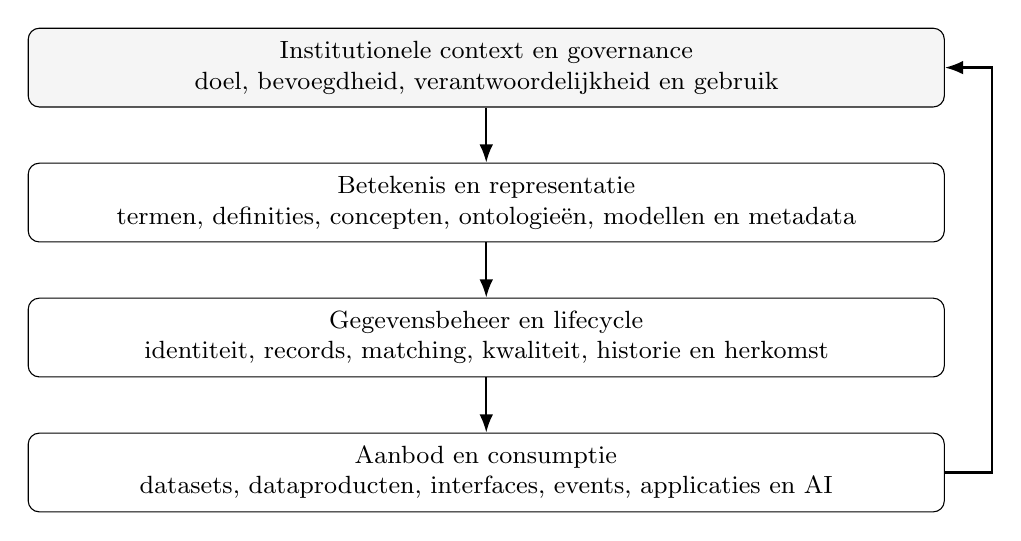
\begin{tikzpicture}[node distance=7mm,box/.style={draw,rounded corners,align=center,text width=11.4cm,minimum height=10mm,font=\small},flow/.style={-{Latex},thick}]
\node[box,fill=black!4] (a) {Institutionele context en governance\\doel, bevoegdheid, verantwoordelijkheid en gebruik};
\node[box,below=of a] (b) {Betekenis en representatie\\termen, definities, concepten, ontologieën, modellen en metadata};
\node[box,below=of b] (c) {Gegevensbeheer en lifecycle\\identiteit, records, matching, kwaliteit, historie en herkomst};
\node[box,below=of c] (d) {Aanbod en consumptie\\datasets, dataproducten, interfaces, events, applicaties en AI};
\draw[flow] (a)--(b);\draw[flow] (b)--(c);\draw[flow] (c)--(d);
\draw[flow] (d.east)--++(.6,0)|-(a.east);
\end{tikzpicture}
\caption{Synthesemodel van de literatuur. De pijlen staan voor analytische afhankelijkheden en terugkoppeling; niet voor verplichte componenten of een gevalideerde architectuur.}
\end{figure}

Drie gevolgtrekkingen zijn centraal. Ten eerste kunnen dezelfde gegevens verschillende rollen hebben: een masterdatarecord kan deel uitmaken van een dataset en via een dataproduct worden aangeboden. Ten tweede zijn verschillende vormen van correctheid te onderscheiden: een schema kan geldig zijn terwijl een referentkoppeling onjuist is. Ten derde moet centrale of federatieve inrichting over meerdere assen worden beoordeeld; plaatsing van data bepaalt niet automatisch gezag of betekenis. Deze gevolgtrekkingen ordenen het corpus zonder één technologie als noodzakelijk te verklaren. \parencite{S47,L12,L22,S32,L24}\claim{RC63}

\subsection{Gedeelde accenten en controverses}
In meerdere geselecteerde bronnen keren organisatiebrede afstemming, gegevenskwaliteit en verantwoordelijkheid terug. Dat ondersteunt een voorzichtige convergentieclaim binnen dit corpus, geen statistisch vastgestelde consensus van het vakgebied. Op het niveau van definities, patronen en roltermen blijft variatie bestaan. Die variatie kan ontstaan door een ander toepassingsdomein, een ander beschouwingsniveau of een andere publicatiedoelstelling. \parencite{L05,L07,L20,P01}\claim{RC64}

Vier spanningen verdienen nadere analyse: uniforme voorkeurswaarden versus legitieme contextverschillen; centrale coördinatie versus domeinautonomie; expliciete semantiek versus modelleer- en onderhoudsinspanning; en kwaliteitscertificering versus feitelijke bruikbaarheid voor een specifieke afnemer. Dit zijn door de synthese geformuleerde spanningsvelden. De paper claimt niet dat de bronnen hierover een georganiseerd debat met twee vaste kampen vormen. \parencite{L19,L20,L23,L13}\claim{RC65}

\section{Research Gaps en open vragen}
Een hiaat in de lokale verzameling is niet hetzelfde als een wetenschappelijke lacune. De volgende agenda onderscheidt vragen die inhoudelijk uit vergelijking volgen van vragen waarvoor vooral extra bronverwerving nodig is. Alle lacuneclaims blijven voorlopig: zij moeten worden ingeperkt wanneer aanvullend werk het vermeende tekort al adresseert.

\begin{longtable}{@{}P{.08\linewidth}P{.37\linewidth}P{.47\linewidth}@{}}
\toprule ID & Open vraag & Type en onderbouwing \\\midrule\endfirsthead
\toprule ID & Open vraag & Type en onderbouwing \\\midrule\endhead
RG01 & Hoe zijn capability-taxonomieën vergelijkbaar zonder bronverschillen te verliezen? & Synthesevraag door uiteenlopende granulariteit in \textcite{L20,L05,P01}; geen bewezen afwezigheid van alle mappings. \\
RG02 & Wanneer levert expliciete semantische formalisering extra waarde boven goed begrips- en metadatabeheer? & Conditionele effectvraag; vroege semantische MDM en kennisgraafliteratuur selecteren geen universeel optimale diepte. \parencite{L18,L13} \\
RG03 & Hoe verhouden MDM-patronen en federatieve governance zich onder gelijke taak- en kostendefinities? & Vergelijkingsvraag; labels en abstractieniveaus verschillen. \parencite{L20,L23,L24} \\
RG04 & Hoe worden identiteit, provenance en institutioneel gezag gezamenlijk geïnterpreteerd? & Integratievraag tussen verschillende constructies; nog geen aangetoond wereldwijd ontbreken van oplossingen. \parencite{L21,S33,S25} \\
RG05 & Welke tijds- en mappinginformatie blijft behouden bij bron- en modelwijzigingen? & Contextgebonden integratievraag vanuit temporele begrippen en metadatamodellen. \parencite{L14,S08,S13} \\
RG06 & Welke effecten heeft contextmetadata bij AI-consumptie van masterdata? & Empirische vervolgbehoefte; RAG- en xLP-resultaten zijn niet zonder meer overdraagbaar. \parencite{L16,L31} \\
RG07 & Wat schrijven volledige toepasselijke ISO/NEN-teksten precies voor? & Toegangslacune van deze review; geen inhoudelijke tekortkoming van de normen. \\
RG08 & Hoe volledig zijn de dekking van FDS, semantic layers, data contracts en AI-agents? & Corpuslacune; gerichte uitbreiding en primaire passagecontrole nodig. \\
\bottomrule
\end{longtable}
Deze agenda draagt claim RC66: zij identificeert onderzoeksvragen en bewijsgrenzen, niet acht reeds bewezen nieuwe research gaps.\claim{RC66}

\section{Discussie}
\subsection{Theoretische bijdrage en alternatieve interpretaties}
De bijdrage is een brongebonden ordening die concepten, capabilities en standaardfuncties verbindt. De paper ontwerpt geen nieuw MDM-product en pretendeert geen nieuwe algemene MDM-theorie. Haar bruikbaarheid ligt in het voorkomen van ongedocumenteerde gelijkstellingen: een identifier wordt geen bewijs van identiteit, een kwaliteitsregel geen waarheidsgarantie en een dataproduct geen nieuw authentiek register.

Een alternatieve lezing is dat de besproken ontwikkelingen vooral bestaande disciplines hernoemen. De aanwezigheid van productdenken en business semantics in vroege MDM-literatuur ondersteunt dat tegenargument gedeeltelijk. Een andere lezing is dat nieuwe technologie de uitvoerbaarheid en schaal van bestaande ideeën verandert. De knowledge graph- en RAG-literatuur maakt technische variatie aannemelijk, maar de huidige review bepaalt niet hoeveel daarvan werkelijk additionele MDM-waarde oplevert. Beide verklaringen blijven dus mogelijk, afhankelijk van de afgebakende capability en context. \parencite{L20,L18,L13,L16}\claim{RC67}

Een derde verklaring voor integratieproblemen is onvoldoende governance of gebrekkige uitvoering van reeds beschikbare standaarden. Dan is een nieuw vocabulaire niet de primaire oplossing. Omgekeerd kunnen bestaande modellen onvoldoende expliciete verbindingen bieden voor een specifieke taak. De analyse moet daarom onderscheid maken tussen ontbrekende specificatie, ontbrekende toepassing, onjuiste mapping en onvoldoende empirisch bewijs. De huidige synthese biedt categorieën voor dat onderscheid, geen algemene diagnose van de Nederlandse overheid. \parencite{L07,S14,S08}\claim{RC68}

\subsection{Praktische betekenis}
Voor organisaties biedt de review een manier om vragen te ordenen voordat een platform of patroon wordt gekozen: welke entiteiten zijn relevant, welke betekenisverschillen zijn legitiem, wie mag beslissen, welke uitkomsten gelden als kwaliteit en welke representaties moeten worden verbonden? Het antwoord kan verschillende combinaties van organisatorische maatregelen en technische voorzieningen opleveren. Een capability-taxonomie hoort daarmee een gesprek en analyse te ondersteunen, niet automatisch een maximaal pakket aan productfuncties te legitimeren.

Voor de Nederlandse context is vooral het onderscheid tussen bronverantwoordelijkheid, publicatieverantwoordelijkheid en afgeleid gebruik relevant. Een dataset of product kan informatie bundelen zonder de status van de onderliggende registraties te vervangen. Dat is een analytische toepassing van de besproken begripsgrenzen, geen juridisch oordeel over een specifieke verwerking. \parencite{S25,S47,S51}

\section{Beperkingen en threats to validity}
\textbf{Selectie en dekking.} Het corpus begon met een ontwerpgerichte selectie en is via gerichte webzoekacties uitgebreid. Selectiebias, beschikbaarheidsbias, zoekmachinerangorde en taalkeuze kunnen de synthese beïnvloeden. De studie heeft geen databasebrede dekking of theoretische verzadiging vastgesteld. Extra downloads verminderen deze beperkingen niet automatisch.

\textbf{Bronkwaliteit en onafhankelijkheid.} Boeken, normen, academische studies, preprints en leveranciersdocumenten ondersteunen verschillende claimtypen. Leveranciersliteratuur is herkenbaar gescheiden, maar vormt voor sommige technische functies een belangrijke bron. Voor die functies ontbreekt soms onafhankelijke vergelijkende onderbouwing. Meerdere bronnen kunnen hetzelfde werk herhalen; documentaantallen mogen daarom niet als onafhankelijk bewijs worden opgeteld.

\textbf{Constructvaliditeit.} De eigen capability-clusters en begripsafbakening kunnen auteursverschillen oversimplificeren. De taxonomie is niet door onafhankelijke beoordelaars gevalideerd. Een expliciete rolvergelijking vermindert terminologische ambiguïteit in de paper, maar bewijst niet dat de voorgestelde categorieën in elke organisatie passend zijn.

\textbf{Toegang en versie.} Officiële catalogi geven geen toegang tot alle norminhoud. Sommige auteursversies bevatten afwijkende jaaraanduidingen of voorlopige publicatiegegevens. De bibliografie vermeldt daarom de gebruikte representatie. Webpagina's en lijststatussen zijn tijdgebonden; de peildatum is geen permanente garantie van actualiteit.

\textbf{Interpretatie en AI-ondersteuning.} Tekstextractie kan tabellen, accenten of paginagrenzen verkeerd weergeven. De AI-ondersteunde analyse kan relaties te snel generaliseren of tegenbewijs missen. Het passage- en claims-register biedt een auditspoor, maar externe vakinhoudelijke controle en waar nodig juridisch-inhoudelijke beoordeling blijven nodig.

\textbf{Externe geldigheid.} Er is geen onderzoek uitgevoerd naar een organisatiepopulatie, een werkende stelselketen of consumentprestaties. Conclusies betreffen de gelezen bronnen. De paper kan geen kostenbesparing, kwaliteitswinst, adoptiegraad of verbeterde AI-interpretatie voor een praktijkcontext vaststellen.

\section{Conclusie}
Binnen het onderzochte corpus verschijnt MDM als een combinatie van entiteitsgericht gegevensbeheer, organisatorische verantwoordelijkheid en technische ondersteuning. Masterdata, referentiedata, metadata, datasets en dataproducten beschrijven verschillende aspecten en kunnen in één aanbod samenkomen. Architectuurpatronen verschillen niet alleen in plaatsing van gegevens, maar ook in schrijfverantwoordelijkheid en afstemming.

De bronvergelijking rechtvaardigt geen algemene claim dat semantiek of productdenken ontbreekt in eerdere MDM-benaderingen. Beide komen al in vroege bronnen voor. De betekenis van nieuwe ontwikkelingen moet daarom worden onderzocht op het niveau van concrete mechanismen, toepassingsvoorwaarden en aantoonbare resultaten. Standaarden verdelen verantwoordelijkheden over terminologie, modellen, metadata, kwaliteit, provenance, aanbod en distributie; hun combinatie vraagt expliciete interpretatie zonder dat daaruit vanzelf een nieuwe architectuur volgt.

De wetenschappelijke opbrengst van deze versie is een controleerbare conceptuele synthese en een begrensde onderzoeksagenda. Verdere corpusuitbreiding, onafhankelijke beoordeling en waar passend empirisch onderzoek moeten vaststellen welke verbindingen praktisch waardevol zijn en waar bestaande kennis al voldoende is. Een prototype vormt geen grondslag voor deze conclusies en is in deze onderzoeksfase niet onderzocht.

\appendix
\section{Brongebonden traceability}\label{app:claims}
De codes in de hoofdtekst verwijzen naar de onderstaande analytische claims. Het machineleesbare register bevat daarnaast bronpassages, grenzen en tegenargumenten. Een geregistreerde claim is geen onafhankelijk gevalideerd resultaat. De vindplaatsen verwijzen naar passages en lokale tekstextracties; voor letterlijke citaten blijft het brondocument leidend.
\small\begin{longtable}{@{}P{.09\linewidth}P{.59\linewidth}P{.24\linewidth}@{}}
\toprule Claim & Analytische uitspraak & Bron-ID\textquotesingle s \\\midrule\endfirsthead
\toprule Claim & Analytische uitspraak & Bron-ID\textquotesingle s \\\midrule\endhead
RC01 & MDM omvat technische en organisatorische beheertaken. & L05, L20 \\
RC02 & Dataproducten en federatieve benaderingen overlappen met MDM zonder ermee samen te vallen. & L12, L24 \\
RC03 & Reviewrapportagerichtlijnen ondersteunen transparantie, geen automatisch systematische dekking. & M01, M02 \\
RC04 & Masterdatadefinities benadrukken domeinentiteiten, hergebruik en afgestemd beheer. & B01, L18, L20 \\
RC05 & Een golden record is geen garantie van juistheid of institutioneel gezag. & L19, P01 \\
RC06 & Vroege MDM-publicaties bevatten semantisch en productgericht denken. & L12, L18, L19, L20, L24 \\
RC07 & Vier theoretische perspectieven bieden een eigen ordening van het corpus. & L07, L08, L15, L21 \\
RC08 & Datacategorieën verschillen in classificatiegrond en zijn niet allemaal exclusief. & L12, L20, S47 \\
RC09 & Capability-taxonomieën verschillen in granulariteit en doel. & L05, L20, P01 \\
RC10 & De lifecycle is een cyclisch analysekader, geen universeel stappenvoorschrift. & L20, P01, P02 \\
RC11 & Patroonlabels verschillen tussen MDM-bronnen. & L20, P01 \\
RC12 & Patroonlabels bepalen niet zelfstandig prestaties of consistentiegaranties. & L24, P01, P02 \\
RC13 & Entity resolution omvat meer dan tekstvergelijking. & L21, L29, L30 \\
RC14 & Identifiergelijkheid, recordgelijkheid en referentidentiteit verschillen. & L08, S38, S39 \\
RC15 & Matching, survivorship en domeinverandering vragen verschillende besluiten. & L08, L22, P01 \\
RC16 & ER-maatstaven kunnen verschillende rangordes opleveren. & L22 \\
RC17 & Datakwaliteit is contextgebonden en multidimensionaal. & L15, L19 \\
RC18 & Kwaliteitsdimensies vereisen expliciete vergelijkingsconventies. & L19, S12 \\
RC19 & Normscope, kwaliteitsmetadata en graafvalidatie hebben verschillende toetsobjecten. & S02, S03, S12, S32, S34 \\
RC20 & Governance adresseert besluitrechten en verantwoordelijkheid. & L07, L20, L27 \\
RC21 & Roltermen vragen bron- en contextgebonden interpretatie. & L07, L20, L23, S51 \\
RC22 & Standaardbeheer is geen volledige data governance. & L07, S23 \\
RC23 & Metadataregistratie onderscheidt conceptuele en representatieconstructies. & S07, S08, S09, S10 \\
RC24 & Een technisch schema bepaalt niet zelfstandig de volledige betekenis. & S08, S11, S14 \\
RC25 & Metadataregistries en catalogi hebben verschillende en overlappende scopes. & S08, S09, S47 \\
RC26 & Term, definitie en begrip zijn te onderscheiden; begrip/concept zijn bronafhankelijk. & S11, S13, S31 \\
RC27 & SKOS, NL-SBB en MIM hebben complementaire en overlappende functies. & S13, S14, S31 \\
RC28 & Bedrijfssemantiek komt aantoonbaar voor in vroegere MDM-literatuur. & B01, L20 \\
RC29 & Gelijke labels garanderen geen gelijke begripsafbakening. & B01, S31 \\
RC30 & EIF-niveaus verschillen van de eigen uitsplitsing van syntaxis en structuur. & S43 \\
RC31 & Conceptuele modellen veronderstellen ontologische categorieën en identiteit. & L08 \\
RC32 & Ontologische modelleerbenaderingen zijn geen universele MDM-vereiste. & L10, S40, S41 \\
RC33 & SKOS-concept, ontologische klasse, objecttype en data-element zijn geen automatische equivalenten. & S08, S13, S31 \\
RC34 & Semantic Web-specificaties vervullen verschillende representatie- en queryfuncties. & S28, S29, S30, S35, S36 \\
RC35 & SMDM is een bestaand antecedent van semantische MDM-integratie. & L18 \\
RC36 & Een formeel valide graaf garandeert geen juiste mapping of broninhoud. & L13, S32 \\
RC37 & PROV-O biedt constructies voor provenance; lineage is hier een werkafbakening. & S33 \\
RC38 & Herkomst is geen zelfstandige waarheids- of bevoegdheidswaarborg. & S25, S33 \\
RC39 & Valid time en transaction time zijn verschillende tijdsbetekenissen. & L14 \\
RC40 & Tijdnotatie en tijdontologie bepalen geen volledig historiebeleid. & P01, S37, S52 \\
RC41 & Documentsoort, normatieve status en empirisch bewijs zijn verschillende assen. & L11, S13, S30, S42 \\
RC42 & Cross-standard relaties vormen een synthese, geen verplichte componentenlijst. & S01, S02, S03, S07, S08, S09, S10, S11, S12, S13, S14, S15, S16, S17, S18, S19, S20, S21, S22, S23, S24, S25, S26, S27, S28, S29, S30, S31, S32, S33, S34, S35, S36, S37, S38, S39, S40, S41, S42, S43, S44, S45, S47, S49, S51, S52 \\
RC43 & Profielrelaties, complementaire metadata en onderzoekersmappings verschillen. & S16, S31, S33, S34, S45, S47 \\
RC44 & Overlap bewijst geen redundantie; scopebeperking bewijst geen wetenschappelijke lacune. & S14, S19, S31 \\
RC45 & Basisregistratieafspraken verbinden kerngegevens met institutionele verantwoordelijkheid. & S25, S26 \\
RC46 & BAG biedt begripsdocumentatie; geen operationele stelselketen is hier onderzocht. & S49 \\
RC47 & Nederlandse standaarden opereren op verschillende abstractieniveaus. & S13, S14, S15, S16, S17 \\
RC48 & Nederlandse lijststatus en technische versie moeten afzonderlijk worden vastgesteld. & F01, F02, F03 \\
RC49 & De FDS-dekking is te beperkt voor reconstructie van operationele afspraken. & S27 \\
RC50 & EIF, Europese wetgeving en SEMIC hebben verschillende functies. & S42, S43, S44 \\
RC51 & FAIR ondersteunt hergebruik en machinegericht gebruik zonder algemene openbaarheidseis. & L11 \\
RC52 & Masterdata en dataproducten beschrijven verschillende aspecten van gegevensaanbod. & L12 \\
RC53 & Masterdata als product is een expliciet eerder gepubliceerd idee. & L20 \\
RC54 & Productmetadata overlappen met catalogus- en registratiemetadata. & S08, S47, S51 \\
RC55 & Data Mesh-principes zijn beschreven in een grijze-literatuurreview. & L23 \\
RC56 & Federatie heeft technische en organisatorische dimensies. & L20, L23, L24 \\
RC57 & API- en eventstandaarden bepalen niet vanzelf domeinbetekenis. & S18, S19, S20, S21, S22 \\
RC58 & Data contracts en API-first zijn hier begrensde onderzoeksoriëntaties. & S19, S47, S51 \\
RC59 & AI kan hulpmiddel en consument van masterdata zijn; xLP is een beperkt voorbeeld. & L29, L31 \\
RC60 & RAG-resultaten bewijzen geen algemeen voordeel van semantische MDM. & L13, L16, S33 \\
RC61 & Machineleesbare epistemische status is een open effect- en representatievraag. & L16, S25, S33 \\
RC62 & Gegevens, representaties, beheer en consumptie vormen een eigen synthesemodel. & L07, L12, L19, L20, S08, S47 \\
RC63 & Gegevensrollen, correctheidsvormen en centralisatie-assen moeten worden onderscheiden. & L12, L22, L24, S32, S47 \\
RC64 & Convergentie in geselecteerde bronnen is geen vastgestelde vakgebiedbrede consensus. & L05, L07, L20, P01 \\
RC65 & Uniformiteit, autonomie, modelleerlast en bruikbaarheid vormen analytische spanningen. & L13, L19, L20, L23 \\
RC66 & De onderzoeksagenda onderscheidt synthesevragen van corpus- en toegangslacunes. & L05, L13, L14, L16, L18, L20, L21, L23, L24, L31, P01, S08, S13, S25, S33 \\
RC67 & Herbenoeming en technische vernieuwing blijven alternatieve interpretaties. & L13, L16, L18, L20 \\
RC68 & Integratieproblemen kunnen door ontbrekende toepassing in plaats van ontbrekende standaarden ontstaan. & L07, S08, S14 \\
\bottomrule\end{longtable}\normalsize

\section{Geselecteerde standaarddocumenten en bewijsgrenzen}
Dit overzicht noemt de gebruikte documentversies; het is geen verklaring van actuele conformiteit of verplichte gezamenlijke toepassing.
\small\begin{longtable}{@{}P{.29\linewidth}P{.22\linewidth}P{.41\linewidth}@{}}
\toprule Document & Gebruikte versie & Niveau en bewijsgrens \\\midrule\endfirsthead
\toprule Document & Gebruikte versie & Niveau en bewijsgrens \\\midrule\endhead
S01 DAMA-DMBOK & DMBOK2 Revised Edition, 2024 & Organisatie en processen. officiële overzichts-/cataloguspagina; beperkte inhoudelijke dekking \\
S02 ISO 8000-100 & 2016 & Uitwisseling. officiële webcontrole; alleen scope \\
S03 ISO 8000-110 & 2021 & Bericht en semantische codering. officiële webcontrole; alleen scope \\
S07 ISO/IEC 11179-3 & 2023; Amd 1:2026 vermeld, inhoud niet geanalyseerd & Meta. officiële webcontrole; alleen scope \\
S08 ISO/IEC 11179-31 & 2023 & Meta en data-element. officiële webcontrole; alleen scope \\
S09 ISO/IEC 11179-33 & 2023 & Meta en collectie. officiële webcontrole; alleen scope \\
S10 ISO/IEC 11179-6 & 2023 & Governance van metadata. officiële webcontrole; alleen scope \\
S11 ISO 704 & 2022 & Terminologie. officiële webcontrole; alleen scope \\
S12 ISO/IEC 25012 & 2008 & Gegevenskwaliteit. officiële webcontrole; alleen scope \\
S13 MIM & 1.2 & Meta; beschouwingsniveaus. geselecteerde passage; geen integrale bronvalidatie \\
S14 NL-SBB & 1.0 & Begrip en terminologie. geselecteerde passage; geen integrale bronvalidatie \\
S15 TOOI & Ontologie 1.6.2 (2025-07-04); lijstdocumentatie 1.3.4 & Domeinsemantiek en referentiedata. geselecteerde passage; geen integrale bronvalidatie \\
S16 DCAT-AP-NL & 3.0 & Dataset; dienst; distributie. geselecteerde passage; geen integrale bronvalidatie \\
S17 NEN 3610 & 2022 & Conceptueel en logisch. officiële overzichts-/cataloguspagina; beperkte inhoudelijke dekking \\
S18 NLGov REST API Design Rules & 2.2.0; Forum vermeldt 2.2 & Interface. geselecteerde passage; geen integrale bronvalidatie \\
S19 OpenAPI Specification & Onderzoeksreferentie 3.1.1; Nederlandse lijst 3.0 & Interface en payloadschema. geselecteerde passage; geen integrale bronvalidatie \\
S20 Digikoppeling & Geen overkoepelend versienummer; REST-API 4.0.1 & Transport; beveiliging; koppelvlak. geselecteerde passage; geen integrale bronvalidatie \\
S21 Federated Service Connectivity (FSC) & Core 2.0.0 & Vertrouwen en infrastructuur. geselecteerde passage; geen integrale bronvalidatie \\
S22 NL GOV profile for CloudEvents & 1.1 & Event envelope. geselecteerde passage; geen integrale bronvalidatie \\
S23 BOMOS & Fundament 3.0.2; andere modules afzonderlijk & Organisatorisch. geselecteerde passage; geen integrale bronvalidatie \\
S24 MDTO & 1.0 & Informatieobject en bewaring. geselecteerde passage; geen integrale bronvalidatie \\
S25 Twaalf eisen basisregistraties & Kamerstuk 26387 nr.18, 2003 & Juridisch en organisatorisch. geselecteerde passage; geen integrale bronvalidatie \\
S26 Stelselafspraken / baseline kwaliteitszorg & Geraadpleegde publicatie 2021; geen release-ID vastgesteld & Stelsel en processen. geselecteerde passage; geen integrale bronvalidatie \\
S27 Federatief Datastelsel (FDS) & Afwegingskader v1, 2025-12-18 & Federatief; organisatie tot dienst. officiële overzichts-/cataloguspagina; beperkte inhoudelijke dekking \\
S28 RDF & 1.1, 2014-02-25 & Representatie. geselecteerde passage; geen integrale bronvalidatie \\
S29 RDFS & 1.1, 2014-02-25 & Schema. geselecteerde passage; geen integrale bronvalidatie \\
S30 OWL & OWL 2, second edition, 2012 & Formele semantiek. geselecteerde passage; geen integrale bronvalidatie \\
S31 SKOS & 2009-08-18 & Begripsrepresentatie. geselecteerde passage; geen integrale bronvalidatie \\
S32 SHACL & 2017-07-20 & Uitvoerbare constraints. geselecteerde passage; geen integrale bronvalidatie \\
S33 PROV-O & 2013-04-30 & Bewering en proces. geselecteerde passage; geen integrale bronvalidatie \\
S34 DQV & 2016-12-15 & Meting en collectie. geselecteerde passage; geen integrale bronvalidatie \\
S35 JSON-LD & 1.1, 2020-07-16 & Representatie en interface. geselecteerde passage; geen integrale bronvalidatie \\
S36 SPARQL & 1.1, 2013-03-21 & Query en protocol. geselecteerde passage; geen integrale bronvalidatie \\
S37 OWL-Time & Recommendation 2017-10-19 & Temporele semantiek. geselecteerde passage; geen integrale bronvalidatie \\
S38 URI / IRI-identificatie & RFC 3986 en 3987, 2005 & Identificatie. geselecteerde passage; geen integrale bronvalidatie \\
S39 Cool URIs for the Semantic Web & 2008-12-03 & Webpublicatie. geselecteerde passage; geen integrale bronvalidatie \\
S40 UFO & Onderzoeksbasis 2005 en 2015; geen release vastgezet & Foundational / domeinonafhankelijk. geselecteerde passage; geen integrale bronvalidatie \\
S41 OntoUML & Geen eenduidige release vastgesteld; onderzoeksbaseline L08 & Conceptueel. geselecteerde passage; geen integrale bronvalidatie \\
S42 Interoperable Europe Act & Verordening (EU) 2024/903 & Juridisch en governance. geselecteerde passage; geen integrale bronvalidatie \\
S43 European Interoperability Framework & 2017, COM(2017)134 & Juridisch; organisatorisch; semantisch; technisch. geselecteerde passage; geen integrale bronvalidatie \\
S44 SEMIC Core Vocabularies & Referenties: Person 2.1.1; Business 2.2.0; Location 2.1.0; Public Org. 2.1.1; geen familie\-versie & Domeinconceptueel en uitwisseling. geselecteerde passage; geen integrale bronvalidatie \\
S45 DCAT-AP & 3.0.1 & Dataset; distributie; dienst. geselecteerde passage; geen integrale bronvalidatie \\
S47 DCAT & 3, 2024-08-22 & Metadata. geselecteerde passage; geen integrale bronvalidatie \\
S49 Catalogus BAG 2018 & 2018, versie 1.0; wijzigingsvoorstellen niet automatisch normatief & Domein; model; registratie. geselecteerde passage; geen integrale bronvalidatie \\
S51 Data Product Ontology (DPROD) & 1.0 Beta 1; document februari 2025, catalogus adoption januari 2025 & Productmetadata en semantische catalogisering. geselecteerde passage; geen integrale bronvalidatie \\
S52 ISO 8601 — Date and time format & Serieoverzicht; 2019-delen vermeld & Datum- en tijdrepresentatie. Officieel web-overzicht; geen volledige norm \\
\bottomrule\end{longtable}\normalsize

\section{Reproduceerbaarheid en onderzoeksbestanden}
De nieuwe paper staat onder \texttt{research/paper/}. Het bronnenregister, de literatuurmatrix, standaardenmatrix, conceptanalyse, het claims-register en het hiatenregister staan onder \texttt{research/evidence/}. Het bestand \texttt{source-extracts.csv} koppelt passages aan bestandshashes; \texttt{paper-selection.csv} onderscheidt aangehaalde bronnen van niet in deze paper gebruikte kandidaten. \texttt{paper-traceability.csv} verbindt onderzoeksvragen, claims, bronnen en papersecties. De dekkingstoets in \texttt{research/analysis/coverage-assessment.md} motiveert de begrensde reikwijdte van deze versie.

De oude ontwerpgerichte paper in de projectroot is geen bron voor de inhoudelijke synthese. Alleen haar onderliggende, afzonderlijk controleerbare bronregistratie is als startpunt hergebruikt. De huidige publicatie is een eerste volledige manuscriptversie, geen afgeronde corpusuitbreiding. De bibliografie onderscheidt de geraadpleegde boekfragmenten en auteursversies van volledige commerciële edities. Normcatalogi ondersteunen slechts de vermelde scope- en editie-informatie.
\printbibliography[title={Referenties}]
\end{document}
